\section{Contamination from Lensing}

We now consider gravitational lensing of the 21--cm signal by the large scale structure, as a source of noise in searches for magnetic fields using the method proposed in this work. We first compute the transverse shear power spectrum and then evaluate the bias it produces for the magnetic--field estimator. We demonstrate that this bias can be expected to be negligible, even for arrays with very futuristic collecting areas of $\sim 100$ km$^2$.

To follow standard lensing notation, we no longer label cartesian coordinate axes with $x$, $y$, and $z$, but rather with numbers, using the convention where directions $1$ and $2$ lie in the plane of the sky, while $3$ lies along the line of sight. Specifically, we use angular coordinates $(\theta_1, \theta_2)$ to denote direction in the sky ${\bf{\widehat n}}$, and $\theta_3$ to denote a comoving interval $r_z/\chi(z)$ along the line of sight, located at redshift $z$, and corresponding to $\Delta z$ interval. As before, we denote variables in Fourier space with tilde, and use $\vec{\ell}\equiv(\ell_1,\ell_2)$ for a conjugate variable of ${\bf{\widehat n}}$. 
 
We start by generalizing the formalism for two--dimensional weak lensing \cite{Weinberg201387} to the three--dimensional case.
In the presence of lensing, coordinate $\theta_i^S$, where $i\in\{1,2,3\}$, maps onto the observed coordinate $\theta_i$ as follows \begin{equation}
\theta_k^S=\theta_k+\frac{\partial\psi}{\partial\theta_k},\ k=1,2,\ \ \ \theta_3^S=\theta_3
\label{eq:lensingmapping}
\end{equation}
where $\psi$ is the lensing potential. The full Jacobian of this coordinate transformation is
\begin{align}
\mathcal{J}_{ij}&=\frac{\partial\theta_i^S}{\partial\theta_j}=\delta_{ij}+\left(\begin{array}{ccc}
\psi_{,11} & \psi_{,12} & \psi_{,13}\\
\psi_{,21} & \psi_{,22} & \psi_{,23}\\
0&0&0
\end{array}\right)_{ij} \nonumber\\
&= I_{ij} + \left(\begin{array}{ccc}
\kappa & 0 & 0\\
0 & \kappa & 0\\
0&0&0
\end{array}\right)_{ij}+\left(\begin{array}{ccc}
\gamma_{11} & \gamma_{12} & \gamma_{13}\\
\gamma_{12} & -\gamma_{11} & \gamma_{23}\\
0&0&0
\end{array}\right)_{ij},\nonumber\\
&(i,j=1,2,3),
\label{eq:lensingtsf}
\end{align}
where $I_{ij}$ represents the unity matrix. In the second step in Eq. (\ref{eq:lensingtsf}), we decomposed the $2\times 2$ upper-left submatrix into a sum of a diagonal matrix and a traceless symmetric matrix $\bm{\gamma}_{2\times 2}$, representing magnification and 2-dimensional shear, respectively. Along with the two transverse shear components, they form into a $3\times 3$ shear matrix $\bm{\gamma}$.

We now switch to Fourier space, where the two-dimensional Fourier transform of the lensing potential reads
\begin{equation}
\widetilde{\psi}(\vec{\ell},z)\equiv\int\psi({\bf\widehat{n}},z)e^{-i\vec{\ell}\cdot{\bf{\widehat n}}}\ d\theta_1 d\theta_2.
\label{eq:potentialFourier}
\end{equation}
The relation between $\psi$ and the Newtonian potential $\Phi$ in a flat universe is
\begin{equation}
\psi({\bf{\widehat n}},z)=
-2\int_0^{\chi(z)}d\chi_1\left[\frac{1}{\chi_1}-\frac{1}{\chi}\right]\Phi({\bf{\widehat n}},\chi_1),
\label{eq:lensingpotential}
\end{equation}
where $\chi_1$ is an integration variable.
Combining Eqs.~(\ref{eq:potentialFourier}) and (\ref{eq:lensingpotential}), we get 
\begin{equation}
\frac{\partial\widetilde{\psi}(\vec{\ell},z)}{\partial\theta_3}=-\frac{2}{\chi(z)}\int_0^{\chi(z)} d\chi_1\widetilde{\Phi}(\vec{\ell},\chi_1).
\label{eq:dpsi_dtheta3}
\end{equation}
From Eqs.~(\ref{eq:dpsi_dtheta3}) and (\ref{eq:lensingtsf}), it follows 
\begin{align}
&\langle\widetilde{\gamma}_{13}^*(\vec{\ell},z)\widetilde{\gamma}_{13}(\vec{\ell}',z')\rangle=\left\langle \ell_1\ell_1'\frac{\widetilde{\psi}^*(\vec{\ell},z)}{\partial\theta_3}\frac{\widetilde{\psi}(\vec{\ell}',z')}{\partial\theta_3}\right\rangle\nonumber\\
&=\frac{4\ell_1\ell_1'}{\chi(z)\chi(z')}\int_0^{\chi(z)}d\chi_1\int_0^{\chi(z')}d\chi_1'\langle\widetilde{\Phi}^*(\vec{\ell},\chi_1)\widetilde{\Phi}(\vec{\ell}',\chi_1')\rangle.
\end{align}

We now define the three--dimensional Fourier transform of the Newtonian potential $\widetilde{\widetilde\Phi}$ through
\begin{equation}
\widetilde{\Phi}(\vec{\ell},\chi)\equiv\int\widetilde{\widetilde{\Phi}}(\vec{\ell},\ell_3)e^{i\ell_3\chi}\frac{d\ell_3}{2\pi},
\end{equation}
where $\ell_3$ is an integration variable. Using this definition, we get
\begin{align}
\langle\widetilde{\Phi}^*(\vec{\ell},\chi)\widetilde{\Phi}(\vec{\ell}',\chi')\rangle=\int\int&\frac{d\ell_3}{2\pi}\frac{d\ell_3'}{2\pi}\langle\widetilde{\widetilde{\Phi}}^*(\vec{\ell},\ell_3)\widetilde{\widetilde{\Phi}}(\vec{\ell}',\ell_3')\rangle\nonumber\\
&\times e^{i(\ell_3'\chi'-\ell_3\chi)}. \label{eq:doubletilde}
\end{align}
Assuming different modes are uncorrelated, we get
\begin{equation}
\bga
\langle\widetilde{\widetilde{\Phi}}^*(\vec{\ell},\ell_3)\widetilde{\widetilde{\Phi}}(\vec{\ell}',\ell_3')\rangle\\
=(2\pi)^3\delta(\ell_3-\ell_3')\delta^2(\vec{\ell}-\vec{\ell}')P_{\Phi}(\sqrt{\ell_3^2+\ell^2}).
\ega
\label{eq:expectation_tildetildephi}
\end{equation}
where
\begin{equation}
\bga
P_{\Phi}(\ell)=\frac{P_{\Phi}(k=\ell/\chi(z))}{\chi(z)^2}\\
=\left[\frac{3}{2}\Omega_mH_0^2(1+z)\right]^2\frac{P_{\delta}(k,z)}{k^4\chi(z)^2},
\ega
\end{equation}
is the angular power spectrum.
Substituting Eq.~(\ref{eq:expectation_tildetildephi}) into (\ref{eq:doubletilde}) and applying Limber approximation $\ell_3\ll\ell$, we obtain
\begin{equation}
\langle\widetilde{\Phi}^*(\vec{\ell},\chi)\widetilde{\Phi}(\vec{\ell}',\chi')\rangle=(2\pi)^2\delta^2(\vec{\ell}-\vec{\ell}')P_{\Phi}(\ell)\delta(\chi'-\chi),
\end{equation}
Thus, for $z\leq z'$,
\beq
\bga
\langle\widetilde{\gamma}_{13}^*(\vec{\ell},z)\widetilde{\gamma}_{13}(\vec{\ell}',z')\rangle\\
=\frac{4}{\chi(z)\chi(z')}\ell_1\ell_1'(2\pi)^2\delta^2(\vec{\ell}-\vec{\ell}')\int_0^{\chi(z)}d\chi_1P_{\Phi}(\ell).
\ega
\label{eq:exp_gamma13}
\eeq

We are interested in calculating the power spectrum $P_{13}(\vec{\ell},z,z')$ of $\gamma_{13}$ components, defined as
\begin{equation}
\bga
\langle\widetilde{\gamma}_{13}^*(\vec{\ell},z)\widetilde{\gamma}_{13}(\vec{\ell}',z')\rangle\equiv(2\pi)^2P_{13}(\vec{\ell},z,z')\delta^2(\vec{\ell}-\vec{\ell}').
\ega
\end{equation}
From Eq.~(\ref{eq:exp_gamma13}) we can express
\begin{equation}
P_{13}(\vec{\ell},z,z')=\frac{4\ell_1^2}{\chi(z)\chi(z')}\int_0^{\chi(z)}d\chi_1P_{\Phi}(\ell),
\end{equation}
where, as before, $\chi_1$ is an integration variable.
Similar result holds for the power spectrum $P_{23}$ of $\gamma_{23}$ component. Finally, the transverse power spectrum $P_t$ can be expressed as 
\beq
\bga
P_t(\ell,z,z')\equiv P_{13}+P_{23}\\
=\frac{4\ell^2}{\chi(z)\chi(z')}\int_0^{\chi(z)}d\chi_1P_{\Phi}(\ell).
\ega
\eeq
If $z=z'$, the above expression simplifies to
\begin{equation}
P_t(\ell,z)=\frac{4\ell^2}{\chi(z)^2}\int_0^{\chi(z)}d\chi_1P_{\Phi}(\ell).
\end{equation}
In Figure \ref{fig:Pt}, we show the transverse power spectra for a range of $z$, for standard cosmology.
\begin{figure}
\centering
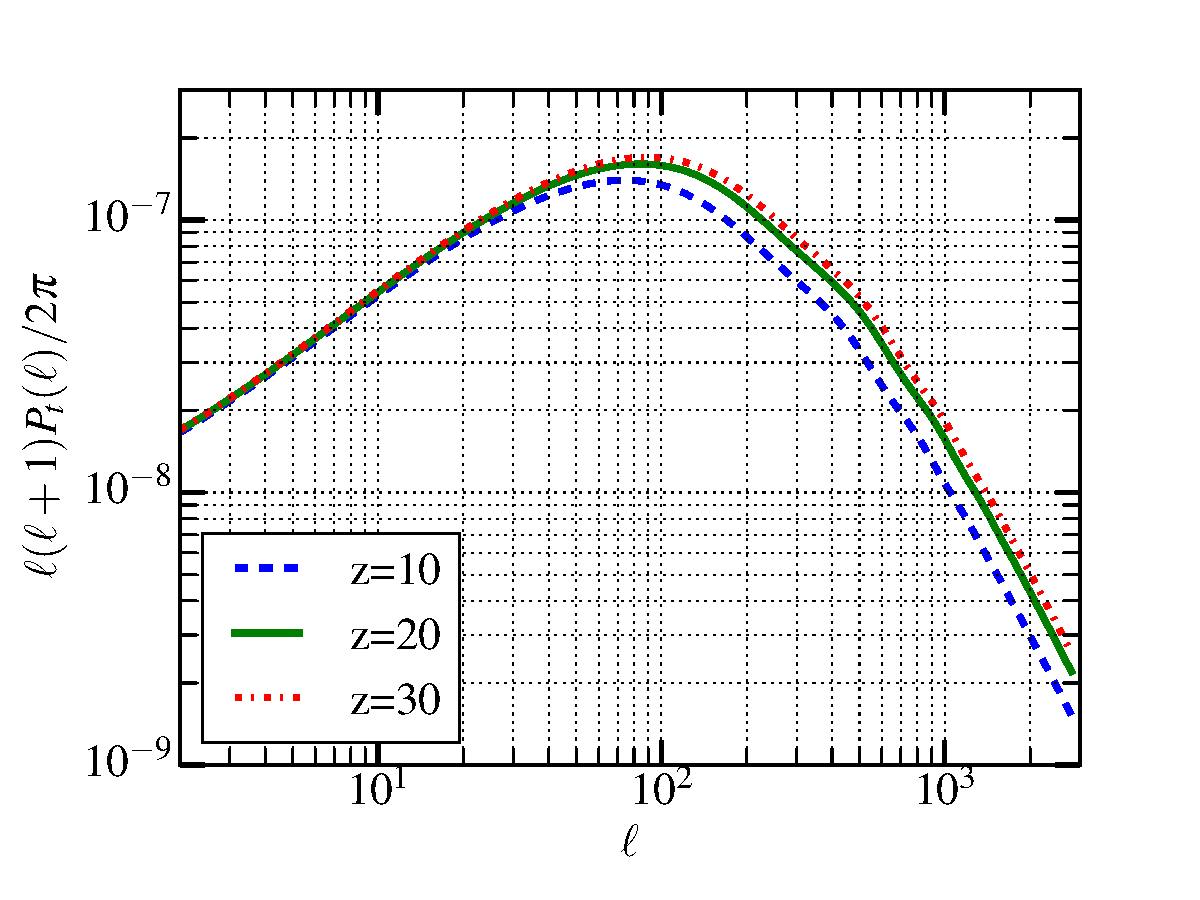
\includegraphics[scale=0.45]{lensing_transverse.pdf}
\caption{The transverse power spectra for sources at redshifts $z=10$, $20$ and $30$, computed for standard cosmology.}
\label{fig:Pt}
\end{figure}

Now that we have computed the transverse power spectrum $P_t$, we move on to evaluating the contamination it produces for the measurement of the magnetic field. Suppose ${\bf{\widehat k}}=(\sin\theta\cos\phi,\sin\theta\sin\phi,\cos\theta)^{\rm T}$, and the line of sight is along the direction 3, ${\bf{\widehat n}}=(0,0,1)^{\rm T}$ in the three-dimensional Cartesian reference frame where $x$, $y$, and $z$ axes correspond to 1, 2, and 3, respectively; $\theta$ is the angle between 3 and ${\bf{\widehat k}}$. Lensing distorts ${\bf{k}}$ into
\begin{align}
\label{eq:distorted_kn}
{\bf{k}}'&=[\mathcal{J}^{-1}]^{\rm T}\cdot{\bf{k}}=\left(1-\frac{2\kappa}{3}\right){\bf{k}}+{\bm{\sigma}}\cdot{\bf{k}}+{\bf{\Omega}}\times{\bf{k}}~,\\
\bm{\sigma}&=\left(\begin{array}{ccc}
-\kappa/3-\gamma_{11} & -\gamma_{12} & -\gamma_{13}/2 \\
-\gamma_{12} & -\kappa/3+\gamma_{11} & -\gamma_{23}/2 \\
-\gamma_{23}/2 & -\gamma_{23}/2 & 2\kappa/3
\end{array}\right)~,\nonumber\\
\bm{\Omega}&=(-\gamma_{23}/2,\gamma_{13}/2,0)^{\rm T}~,\nonumber
\end{align}
where the first term only changes the magnitude of ${\bf{k}}$, the third term only changes the direction of ${\bf{k}}$, while the second term contributes to both. To the first order, the magnitude is changed by
\begin{equation}
\frac{k'-k}{k}=-\frac{2\kappa}{3}+\hat{\bf{k}}\cdot\bm{\sigma}\cdot\hat{\bf{k}}~.
\end{equation}
For conciseness, we define
\begin{equation}
C\equiv 26.4\ {\rm mK}\ \left(1-\frac{T_\gamma}{T_{\rm s,0}}\right)x_{\rm 1s,0}\left(\frac{1+z}{10}\right)^{1/2},
\end{equation}
then the $\mathcal{O}$(optical depth) solution to brightness temperature is given by
\begin{equation}
\delta\tilde{T}_{\rm b}({\bf{k}},\widehat{\bf{n}})=C \tilde{\delta}({\bf{k}})\left(1+(\widehat{\bf{k}}\cdot\widehat{\bf{n}})^2\right).
\end{equation}
From Eq. (\ref{eq:distorted_kn}), in the presence of lensing, this quantity becomes
\beq
\bga
\delta\tilde{T}_{\rm b,lensed}({\bf{k}},\widehat{\bf{n}})=\frac{1}{\det(\mathcal{J})}\delta\tilde{T}_{\rm b}\left({\bf{k}}'\right) \simeq \\
\delta\tilde{T}_{\rm b,unlensed}({\bf{k}},\widehat{\bf{n}})(1-2\kappa) +C\left\lbrace \tilde{\delta}({\bf{k}})2(\widehat{\bf{k}}\cdot\widehat{{\bf{n}}})\left[\widehat{{\bf{n}}}\cdot\bm{\sigma}\cdot\widehat{{\bf{k}}}\right.\right. \\
\left.\left.-(\widehat{\bf{k}}\cdot\widehat{{\bf{n}}})(\widehat{\bf{k}}\cdot\bm{\sigma}\cdot\widehat{{\bf{k}}})+(\bm{\Omega}\times\widehat{{\bf{k}}})\cdot\widehat{{\bf{n}}}\right]\right.\\
\left.+\left(-\frac{2\kappa}{3}{\bf{k}}+\bm{\sigma}\cdot{\bf{k}}
+\bm{\Omega}\times{\bf{k}}\right)\cdot\bm{\nabla}_{\bf{k}}\tilde{\delta}({\bf{k}})\left[1+(\widehat{\bf{k}}\cdot\widehat{{\bf{n}}})^2\right]\right\rbrace
\ega
\eeq
The observable is the two-point correlation function of this brightness temperature, which, with all terms up to first order in the lensing potential included, is given by
\beq
\bga
P_{T_{\rm b}}({\bf{k}})=C^2 P_{\delta}(k)\left(1+(\widehat{\bf{k}}\cdot\widehat{{\bf{n}}})^2\right) \times\\
\left\lbrace \left(1+(\widehat{\bf{k}}\cdot\widehat{{\bf{n}}})^2\right) \left[1-2\kappa\left(1+\frac{n_{\rm eff}}{3}\right)+n_{\rm eff}(\widehat{\bf{k}}\cdot\bm{\sigma}\cdot\widehat{{\bf{k}}})\right]\right.\\
\left. + 4(\widehat{\bf{k}}\cdot\widehat{{\bf{n}}})\left(\left[\widehat{\bf{n}}-(\widehat{\bf{k}}\cdot\widehat{{\bf{n}}})\widehat{\bf{k}}\right]\cdot\bm{\sigma}\cdot\widehat{\bf{k}}+(\bm{\Omega}\times\widehat{\bf{k}})\cdot\widehat{\bf{n}}\right)\right\rbrace,
\label{eq:Tb_power}
\ega
\eeq
where $n_{\rm eff}(k,z)\equiv \partial\ln P(k,z)/\partial\ln k$ is the effective spectral index (which is a function of the range of $k$ and redshift of interest; in our case, $n_{\rm eff}\sim -2.15$).

From Eq. (137) of \cite{2014arXiv1410.2250V}, we obtain the power spectrum in the precence of the magnetic field
\beq
\bga
P_{T_{{\rm b},{\bf{B}}}}({\bf{k}})=C^2 P_{\delta}(k)\left(1+(\widehat{\bf{k}}\cdot\widehat{{\bf{n}}})^2\right) \times\\
\left\lbrace \left(1+(\widehat{\bf{k}}\cdot\widehat{{\bf{n}}})^2\right) + 1.353\times 10^{16}\left(\frac{1+z}{10}\right)^{-1/2}\right. \\
\left.\times \frac{T_{\gamma}}{T_{\rm s,0}}\frac{x_{\rm 1s,0}}{(1+x_{\alpha,(2)}+x_{c,(2)})^2}\left[{\bf{B}}_{\rm G}\cdot(\widehat{\bf{k}}\times\widehat{{\bf{n}}})\right](\widehat{\bf{k}}\cdot\widehat{{\bf{n}}})\right\rbrace,
\label{eq:Tbmag_power}
\ega
\eeq
where ${\bf{B}}_{\rm G}$ is the physical magnetic field in units of Gauss. Suppose the magnetic field is on the $1-2$ plane, ${\bf{B}}=(B_x,B_y,0)$ and define $B_{\pm}=\mp(1/\sqrt{2})(B_x\pm iB_y)$, the last term in the last set of braces in Eq. (\ref{eq:Tbmag_power}) has the following angular dependence
\beq
\bga
\left(1+(\widehat{\bf{k}}\cdot\widehat{{\bf{n}}})^2\right)\left[{\bf{B}}\cdot(\widehat{\bf{k}}\times\widehat{{\bf{n}}})\right](\widehat{\bf{k}}\cdot\widehat{{\bf{n}}})\\
=\frac{4i}{7}\sqrt{\frac{\pi}{15}}\left[B_-\left(5Y_{21}(\theta,\phi)+\sqrt{\frac{2}{3}}Y_{41}(\theta,\phi)\right)\right.\\
\left. -B_{+}\left(5Y_{2-1}(\theta,\phi)+\sqrt{\frac{2}{3}}Y_{4-1}(\theta,\phi)\right)\right]
\ega
\eeq
Hence the terms that mimic some arbitrary magnetic field in the lensing case are those that produce $Y_{2\pm 1}$ and $Y_{4\pm 1}$ spherical harmonics in the observed brightness temperature power spectrum. The spherical harmonic decompositions of the terms involving $(\widehat{\bf{k}}\cdot\bm{\sigma}\cdot\widehat{{\bf{k}}})$, $(\widehat{\bf{n}}\cdot\bm{\sigma}\cdot\widehat{{\bf{k}}})$, and $(\bm{\Omega}\cdot\widehat{\bf{k}})\times\widehat{\bf{n}}$ in Eq. (\ref{eq:Tb_power}) have parts that are not symmetric around $\widehat{\bf{n}}$, such as $Y_{2\pm 1}$,  $Y_{4\pm 1}$ and  $Y_{6\pm 1}$ terms. Since the $Y_{2\pm 1}$ harmonics of the brightness temperature power spectrum represent the lowest order of the asymmetry, we only use them to study magnetic fields for now. Matching all the contributions, the "equivalent comoving magnetic field" due to lensing is
\beq
\bga
{\bf{B}}^{(\rm lens)}=1.577\times 10^{-18}{\rm G}\ x_{\rm 1s,0}^{-1}\left(\frac{T_{\gamma}}{T_s}\right)^{-1}\left(\frac{10}{1+z}\right)^{3/2}\\
\times(1+x_{\alpha,(2)}+x_{c,(2)})^2\left(1+\frac{11}{16}n_{\rm eff}(k,z)\right)(-\gamma_{23},\gamma_{13},0)^{\rm T}\\
\equiv\alpha(-\gamma_{23},\gamma_{13},0)^{\rm T}~.
\ega
\eeq

Finally, the lensing contamination to the magnetic--field reconstruction is
\begin{equation}
P_B^{(\text{lens})}(\ell)=P^{(\text{lens})}_{B_x}+P^{(\text{lens})}_{B_y}=\alpha^2 (P_{\gamma_{13}}+P_{\gamma_{23}})=\alpha^2 P_t(\ell),
\end{equation}
and the root--mean--square (rms) of the total contamination is
\beq
\Delta_B^{(\text{lens})}(\ell)=\sqrt{\frac{\ell(\ell+1)}{2\pi}P_B^{(\text{lens})}(\ell)}.
\eeq
A survey of size $\Omega_{\rm survey}=1{\rm sr}$ corresponds to the largest scale of $\ell\sim 6$, which relates to the lensing potential fluctuations of comoving scale $k_\Phi=\ell/D(z)\sim 5\times 10^{-4}{\rm Mpc}^{-1}$ at redshift $z\sim 20$. We choose this $\ell$ since it determines the average variance of transverse shear power spectrum in the survey region. This scale is much larger than the scale of matter density fluctuations ($k_\delta\sim 1$) that contribute to the signals, so that our weak lensing approximation is valid.

We show numerical results for the rms contamination in Figure \ref{fig:lensing_B}, calculated with and without the de--lensing procedure (using CMB lensing measurements), with little difference found between the two cases. Comparing this result to Figure \ref{fig:Bsat}, we can see that the contamination due to lensing shear remains below the projected sensitivities even for the case of futuristic array sizes.
\begin{figure}[h]
\centering
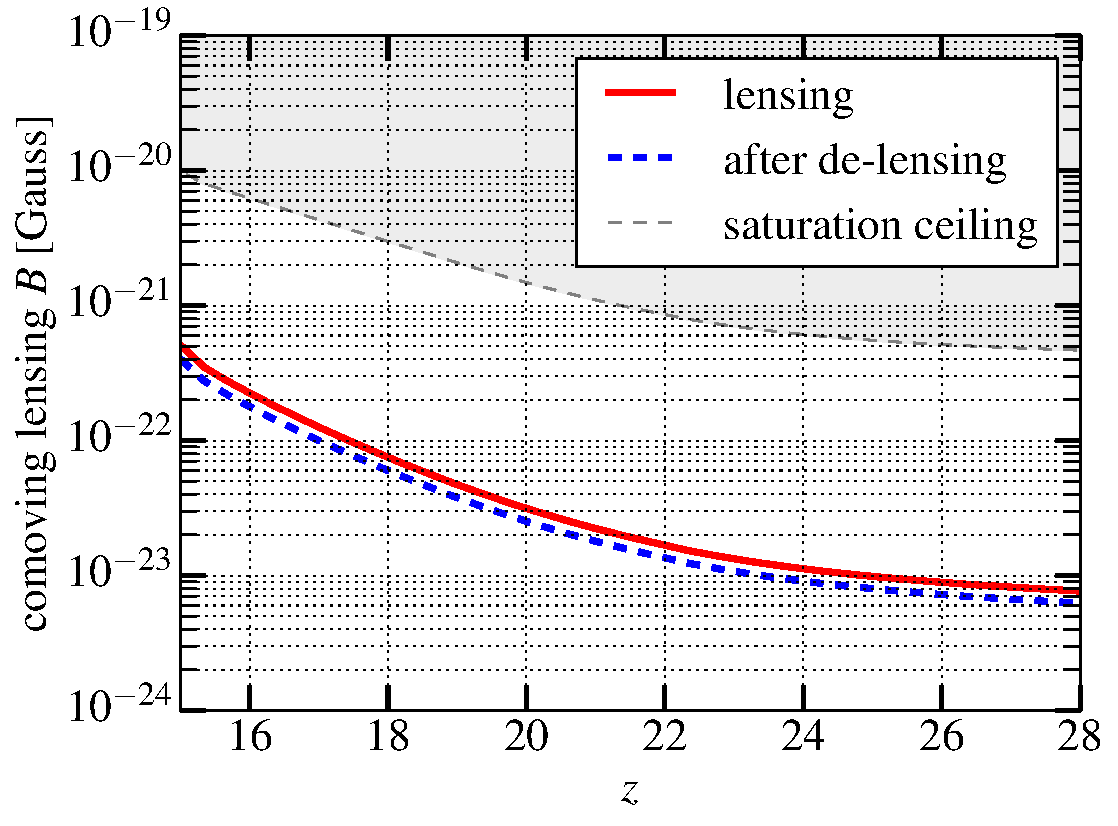
\includegraphics[scale=0.4]{delensingB.pdf}
\caption{Shown is the $1\sigma$ lensing--shear contamination to the measurement of the magnetic field, using the method discussed in this work. Contamination before (solid red line) and after (dashed blue line) the de--lensing procedure, is presented as a function of redshift. Saturation ceiling is denoted by the shaded region above the thin dashed line. Comparison with Figure \ref{fig:Bsat} reveals that lensing is below the projected sensitivity for all array sizes considered in this work.}
\label{fig:lensing_B}
\end{figure}
%Note that the scale of the relevant matter fluctuations is determined by the resolution of the experiment from $k\sim \frac{2\pi L}{\lambda_0(1+z)D}\sim 1$, which corresponds to $n_{\rm eff}\sim -2.274$ in our case.

